%----------------------------------------------------------------------------------------
\section{Design of a Wireless Sensor Networking Test-Bed}
%------------------------------------------------------------------
\subsection{Thesis subject context}
This thesis is actually part of a bigger project with as goal the creation of a WSN test-bed, the storage of sensor data to a cloud database and the development of a graphical web-application to visualize, configure and control the WSN test-bed.

\subsection{WSN Test-Bed and gateway to extract the data}
\label{lab2}
The purpose of this thesis is to create a WSN test-bed, covering part of the Group T, campus Vesalius, building. So the main focus of this thesis subject, is to sample the data via the nodes and to extract that information out of the network, indicated in green on figure \ref{fig:thesis}. This test-bed consists of at least five nodes, including one weather station. The weather station will be deployed on the roof of Group T, campus Vesalius. The other nodes will be installed amongst the classrooms of the campus\footnote{Most likely, this will be in rooms V200, V6.01, V10.01 and V11.01.} and the gateway will be installed at module 14. We will then, for example, monitor the temperature, humidity and CO$_{2}$ values at those rooms. This data acquisition can happen at intervals between one and several minutes, depending on the user requirements entered through the web interface and on the intended battery life time of the node.\\
In the end, this test-bed can be used as a lab environment for educational-related projects or can form the base for future research projects, for example by extending the network with actuator nodes. The test-bed will thus represent as a stable network of sensing nodes and it will be very easy to integrate new nodes to the network.\\
The gateway developed to extract the data from the WSN test-bed is a middleware communication layer supporting sensor discovery, sensor state tracking and event or query-based data acquisition. Since privileged web-interface users have the possibility to communicate directly to the WSN, the gateway also runs a web service that can be contacted by clients via a web browser.\\
\noindent
ZigBee defines three logical device roles, differentiated in the network layer (table \ref{fig:roles} from \defcitealias{DYNAMIC}{Dynamic C: An Introduction to ZigBee User Manual, 2008}\citepalias{DYNAMIC} in appendix \ref{AppendixA} compares the device roles in detail). Each network must have one and only one \textit{coordinator}, responsible for establishing the network. In the test-bed this is the XBee radio installed at the gateway. A \textit{router} node has the second most complex device role and can also allow other nodes to join the network by becoming its parent. The third, simplest and cheapest device role is the \textit{end device}.  End devices don't have the parenting functionalities and thus cannot allow other nodes to join the network via them. In a typical ZigBee network end devices are also the only nodes which are allowed to sleep. Coordinator and routers are expected to be net-powered and end devices can be battery powered.\\
ZigBee extends the star and basic peer-to-peer topologies supported by IEEE 802.15.4 with the mesh and cluster tree topology. The test-bed uses a mesh topology, in which coordinator and routers are responsible for route discovery, so there are no static routes.  Figure \ref{fig:network2} displays a basic star, tree and mesh topology.
\begin{figure}[htbp]
\centering
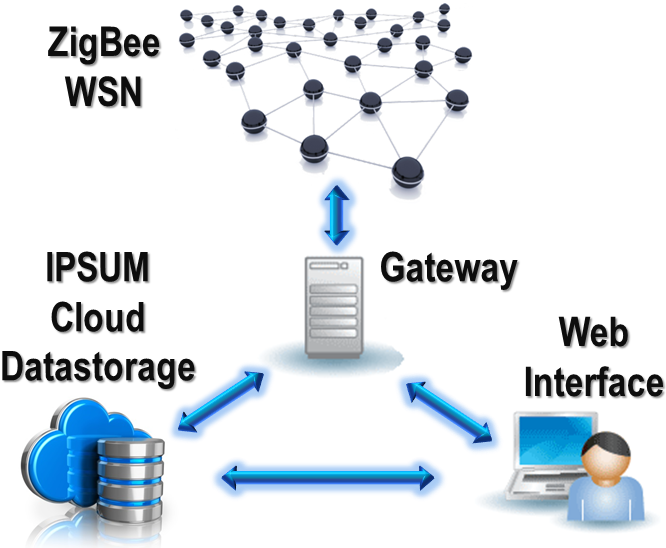
\includegraphics[width=0.48\textwidth]{thesis}
\caption{The context of the WSN Test-Bed}
\label{fig:thesis}
\end{figure}
\begin{figure}[htbp]
\centering
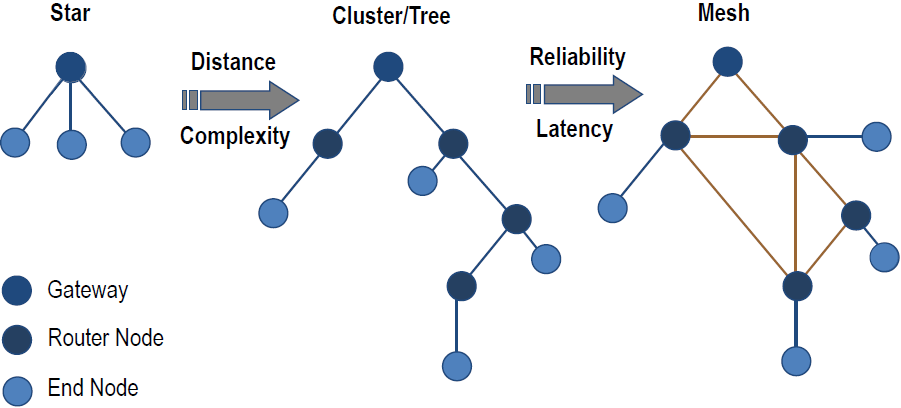
\includegraphics[width=0.48\textwidth]{network2}
\caption{The basic network topologies}
\label{fig:network2}
\end{figure}\\
\noindent
%Since wireless sensor nodes are battery powered also the power consumption of these nodes has to be examined thoroughly to try and function for as long as possible without having to recharge the batteries. 
\subsection{Data storage} 
For reliable sensor data storage the gateway will forward the data to Ipsum. This is a cloud storage system developed at Group T as a master thesis of Ruben Taqc. Ipsum is already in use to log data coming from other sensors and has received a few updates to better support the WSN test-bed.\\
For a WSN it is crucial that data storage happens correctly at all times. No data can be lost. So if Ipsum is unreachable, the gateway will temporally store the incoming data.

\subsection{Web-Interface}
The web interface of the WSN test-bed is the master thesis of Matthias Verhelst and provides the user with 2D/3D models indicating the location of the sensor nodes. By selecting a sensor, the user will), depending on his privileges, will have access to the current state of the node, will be able to change the node's configuration and will be able to send messages (requests) to the node. For non-privileged users the web interface will provide data via Ipsum. The web application also provides the service to add or delete sensors and to define their service capabilities, e.g. the sensor layout of a certain node.

\subsection{Requirements}
In a first stage, this work aimed to design, implement and configure the ZigBee WSN test-bed and the communication layer to extract the sensor data. The most important aspect of this part were network stability, network topologies and network coverage. The network must monitor sensors at default intervals by all means and this data is not to be lost. Nodes must be able to self-recover when they were temporarily unable to join the network.\\
The network must also support additional services such as sensor discovery, sensor state tracking and event-based sensor acquisition. A privileged user of the web interface must for example be able to set different time settings. This can be for all sensors of a certain type or for all sensors of a certain node. This means a node may, for example, have to sample different sensors at different intervals. These settings must be handled by the gateway and stored into the nodes.  To assure overall network stability, network security aspects must be taken into account as well.
%\vfill 